\chapter{अभिक्रिया की एन्ट्रॉपी और मुक्त ऊर्जा}\label{ch:b2:reaction-free-energy}

खिलाड़ियों के ठंडे पैक में पानी की एक थैली और कुछ चम्मच अमोनियम
नाइट्रेट होता है। उसे दबाइए, भीतर की थैली फटती है, लवण घुलता है, और कुछ ही
सेकंडों में पैक इतना ठंडा हो जाता है कि मोच खाए टखने को आराम दे सके। यह विलयन
ऊष्मा अवशोषित करता है --- यह \omterm{def:b2:reaction-enthalpy:exothermic}{ऊष्माशोषी} है --- फिर भी अपने आप, पूर्णता तक
चलता है। पिछले अध्याय की एन्थैल्पी पूरी कहानी नहीं हो सकती:
अभिक्रिया केवल ``ऊष्मा की ढलान पर नीचे'' नहीं जाती। लुप्त राशि
एन्ट्रॉपी है, जिसे भौतिकी में मिला ऊष्मागतिकी का द्वितीय नियम हर स्वतः
परिवर्तन का निर्णायक बनाता है। यह अध्याय एन्ट्रॉपियों को सारणीबद्ध करता है,
अभिक्रिया की एन्ट्रॉपी परिकलित करता है, और एन्थैल्पी तथा एन्ट्रॉपी को एक ही
फलन, \omterm{def:b2:reaction-free-energy:gibbs-energy}{गिब्स ऊर्जा}, में जोड़ता है, जिसका अभिक्रिया-अवकलज नियत ताप और दाब पर
हर अभिक्रिया की दिशा तय करता है।

\begin{recall}
भौतिकी से: द्वितीय नियम। हर निकाय का एक अवस्था फलन होता है, उसकी
एन्ट्रॉपी $S$ (विस्तीर्ण); बंद निकाय के किसी रूपांतरण में $\dd S =
\delta Q/T_{\text{बाह्य}} + \delta S_{\text{c}}$, जहाँ उत्पन्न एन्ट्रॉपी
$\delta S_{\text{c}}$ उत्क्रमणीय परिवर्तन के लिए शून्य है और अन्यथा
धनात्मक; नियत संघटन वाले बंद निकाय के लिए $\dd U = T\dd S -
p\dd V$। \Cref{ch:b2:reaction-enthalpy}: \omterm{def:b2:reaction-enthalpy:reaction-quantity}{अभिक्रिया राशियाँ} $\Delta_r X =
(\partial X/\partial\xi)_{T,p}$ और \omterm{def:b2:reaction-enthalpy:standard-reaction-enthalpy}{मानक अभिक्रिया एन्थैल्पियाँ}। प्रथम वर्ष के
खंड ने, ``द्वितीय नियम से निकलने वाले'' नियमों के रूप में, कहा था कि
अभिक्रिया $Q = K^\circ$ होने तक आगे बढ़ती है; यह अध्याय और अगले दो उन्हें
व्युत्पन्न करते हैं।
\end{recall}

\begin{omfigure}
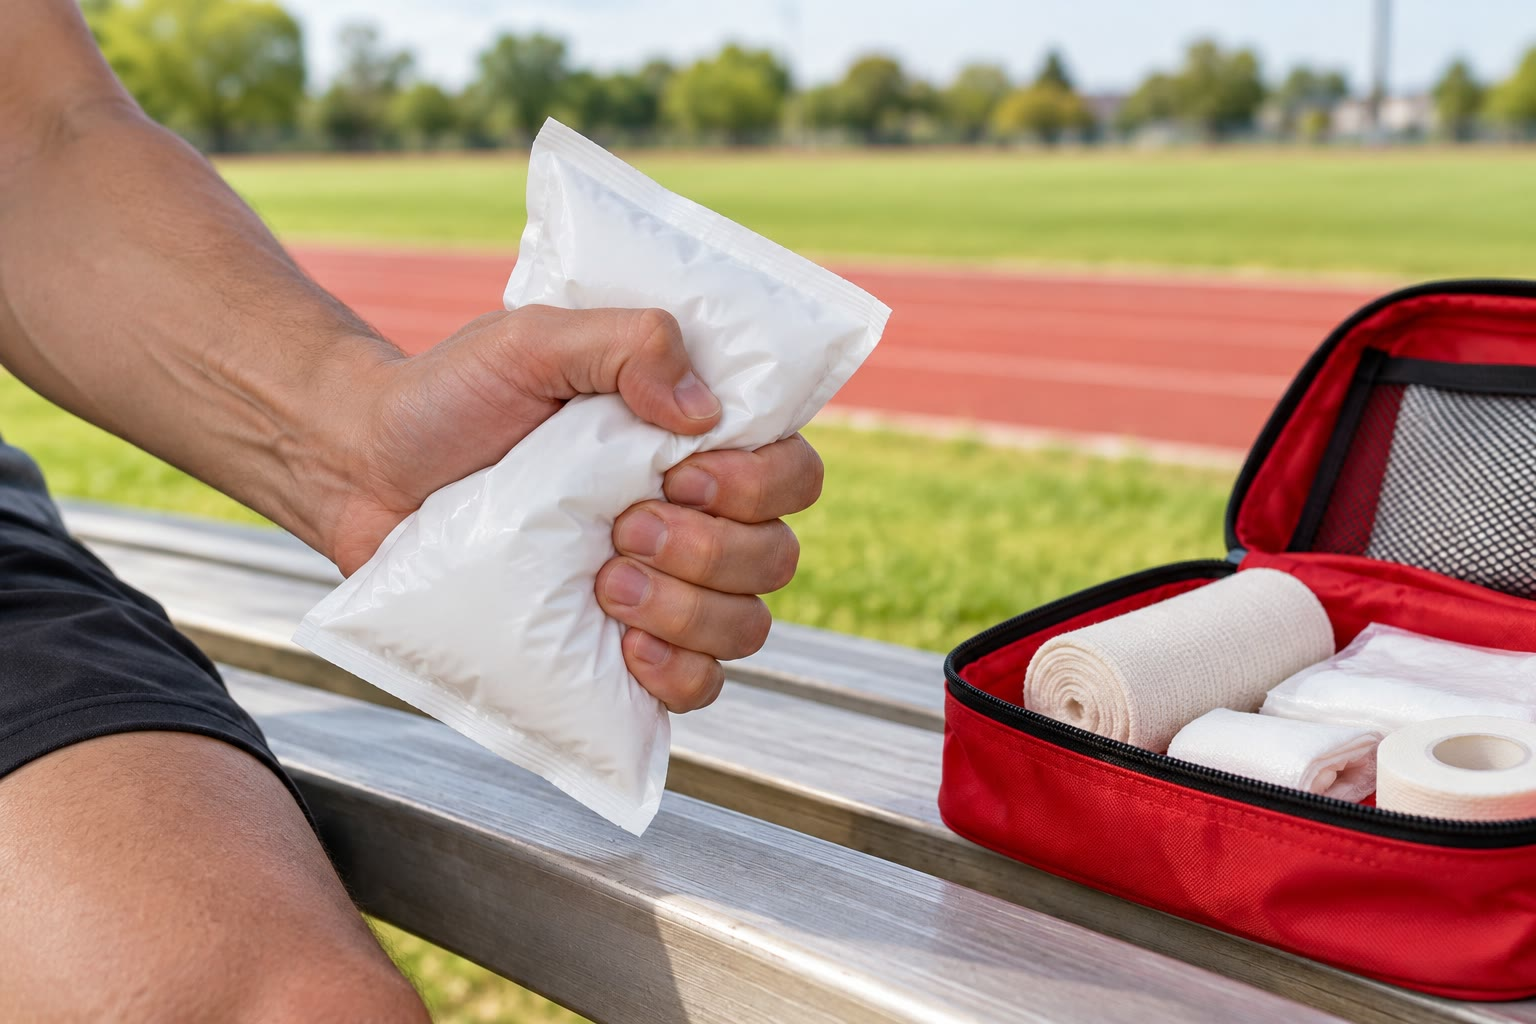
\includegraphics[width=0.55\linewidth]{images/book3/ai/b2-02-cold-pack.jpg}

{\small ठंडा पैक: जब उसकी भीतरी थैली तोड़ी जाती है, तो अमोनियम नाइट्रेट
पानी में घुलता है और पैक ठंडा हो जाता है। यह विलयन \omterm{def:b2:reaction-enthalpy:exothermic}{ऊष्माशोषी} और
स्वतः है; उसकी एन्ट्रॉपी कारण बताती है (\cref{ex:b2:reaction-free-energy:cold-pack})।}
\end{omfigure}

\section{मानक एन्ट्रॉपियाँ और तृतीय नियम}

एन्थैल्पी के विपरीत, एन्ट्रॉपी का एक प्राकृतिक शून्य होता है।

\begin{theorem}[ऊष्मागतिकी का तृतीय नियम]\label{thm:b2:reaction-free-energy:third-law}
किसी शुद्ध, पूर्णतः व्यवस्थित क्रिस्टल की एन्ट्रॉपी शून्य की ओर प्रवृत्त होती है
जब उसका ताप \qty{0}{K} की ओर प्रवृत्त होता है।
\end{theorem}
\admitted

\begin{remark}[शून्य कहाँ से आता है]\label{rem:b2:reaction-free-energy:third-law}
वाल्टर नेर्न्स्ट ने 1906 में कहा कि संघनित प्रावस्थाओं के बीच \omterm{def:b2:reaction-free-energy:reaction-entropy}{अभिक्रिया
एन्ट्रॉपियाँ} $T \to 0$ होने पर लुप्त हो जाती हैं; माक्स प्लांक ने इसे ऊपर के
कथन का तीखा रूप दिया। इसका मूल सांख्यिकीय है: एन्ट्रॉपी उन सूक्ष्म
विन्यासों को गिनती है जो निकाय की अवस्था के अनुरूप हैं, और \qty{0}{K} पर
पूर्ण क्रिस्टल का केवल एक विन्यास होता है। यह गिनती तृतीय वर्ष के खंड में,
विभाजन फलनों के साथ, की जाती है।
\end{remark}

\begin{definition}[मानक मोलर एन्ट्रॉपी]\label{def:b2:reaction-free-energy:standard-entropy}
किसी पदार्थ की \emph{मानक मोलर एन्ट्रॉपी}\index{मानक मोलर एन्ट्रॉपी}
$S^\circ_m(T)$ ताप $T$ पर उसकी मानक अवस्था में उसके एक मोल की
एन्ट्रॉपी है, जिसका शून्य तृतीय नियम वाला है।
$\Delta_f H^\circ$ के विपरीत, यह एक निरपेक्ष राशि है, जो तत्वों सहित हर
पदार्थ के लिए धनात्मक होती है।
\end{definition}

\begin{proposition}[ऊष्मा धारिताओं से निरपेक्ष एन्ट्रॉपी]\label{prop:b2:reaction-free-energy:absolute-entropy}
किसी पदार्थ को नियत दाब $p^\circ$ पर \qty{0}{K} से $T$ तक गर्म करने पर,
\[
  S^\circ_m(T) = \int_0^T\frac{C^\circ_{p,m}(T')}{T'}\,\dd T' +
  \sum_{\text{संक्रमण}}\frac{\Delta_{\text{संक्रमण}}H^\circ}{T_{\text{संक्रमण}}} ,
\]
जहाँ समाकल हर प्रावस्था में उसके ताप-परिसर पर लिया जाता है।
\end{proposition}

\begin{proof}
पदार्थ को नियत दाब पर उत्क्रमणीय रूप से गर्म कीजिए: $\delta S_{\text{c}} =
0$ और $\delta Q = \dd H = C_p\,\dd T$, अतः $\dd S = C_p\,\dd T/T$। किसी
संक्रमण (गलन, क्वथन) पर ताप $T_{\text{संक्रमण}}$ पर बना रहता है
जबकि ऊष्मा $\Delta_{\text{संक्रमण}}H$ उत्क्रमणीय रूप से प्राप्त होती है: एन्ट्रॉपी
$\Delta_{\text{संक्रमण}}H/T_{\text{संक्रमण}}$ से उछलती है। तृतीय नियम वाले शून्य से
आरंभ करके सभी खंडों को जोड़िए।
\end{proof}

\begin{omfigure}
\begin{tikzpicture}
\begin{axis}[
  width=0.8\linewidth, height=6.2cm, xmin=0, xmax=1500, ymin=0, ymax=210,
  axis x line=bottom, axis y line=left, xlabel={$T$ (K)},
  ylabel={ज़िंक की $S^\circ_m$ (\unit{J/(K.mol)})},
  xtick={0,250,500,750,1000,1250,1500},
  tick label style={font=\small}, label style={font=\small}, clip=false]
\addplot[omDef, very thick, smooth] table[x=T, y=S] {figdata/out/bachelor-2-standard-entropy-solid.dat};
\addplot[omProp, very thick] table[x=T, y=S] {figdata/out/bachelor-2-standard-entropy-liquid.dat};
\addplot[omThm, very thick] table[x=T, y=S] {figdata/out/bachelor-2-standard-entropy-gas.dat};
\draw[densely dashed, gray] (axis cs:692.73,64.6) -- (axis cs:692.73,75.2);
\draw[densely dashed, gray] (axis cs:1180.2,91.9) -- (axis cs:1180.2,189.6);
\node[omDef, font=\small, anchor=south east] at (axis cs:600,60) {ठोस};
\node[omProp, font=\small, anchor=north west] at (axis cs:850,78) {द्रव};
\node[omThm, font=\small, anchor=south] at (axis cs:1350,192) {गैस};
\node[font=\scriptsize, anchor=west, align=left] at (axis cs:700,110) {गलन, $+10.6$\\ \qty{692.7}{K} पर};
\node[font=\scriptsize, anchor=east, align=right] at (axis cs:1170,150) {क्वथन,\\ $+97.7$\\ \qty{1180.2}{K} पर};
\end{axis}
\end{tikzpicture}

{\small तृतीय नियम वाले शून्य से ज़िंक की \omterm{def:b2:reaction-free-energy:standard-entropy}{मानक मोलर एन्ट्रॉपी}। धातु के
ऊष्मा संचित करने के साथ यह ताप के साथ बढ़ती है, फिर गलनांक पर
$\Delta_{\text{गलन}}H/T_{\text{गलन}}$ से उछलती है और, कहीं अधिक, क्वथनांक
पर $\Delta_{\text{वाष्पन}}H/T_b$ से: गैस द्रव से कहीं अधिक
अव्यवस्थित होती है।}
% ledger: s0T:Zn_crl.0, s0T:Zn_crl.298.15, s0T:Zn_cr.692, s0T:Zn_l.692, s0T:Zn_l.1180, s0T:Zn_g.1180, hT:Zn_cr.692, hT:Zn_l.692, hT:Zn_l.1180, hT:Zn_g.1180, dfh:Zn_g (curve in figdata/bachelor-2/standard-entropy.py)
\end{omfigure}

चित्र परिमाण की ऐसी कोटियाँ देता है जो याद रखने योग्य हैं। कमरे के
ताप पर कोई धातु या कठोर क्रिस्टल कुछ दसियों
\unit{J/(K.mol)} रखता है, द्रव लगभग सौ, गैस एक सौ से तीन सौ;
गलन थोड़ा जोड़ता है, क्वथन बहुत। इस खंड में प्रयुक्त \omterm{def:b2:reaction-free-energy:standard-entropy}{मानक मोलर एन्ट्रॉपियाँ}
संभवन एन्थैल्पियों के साथ सारणीबद्ध हैं।

\section{अभिक्रिया एन्ट्रॉपी}

\begin{definition}[अभिक्रिया एन्ट्रॉपी]\label{def:b2:reaction-free-energy:reaction-entropy}
\emph{अभिक्रिया एन्ट्रॉपी}\index{अभिक्रिया एन्ट्रॉपी} $\Delta_r S =
(\partial S/\partial\xi)_{T,p}$ है, और \emph{मानक अभिक्रिया
एन्ट्रॉपी}\index{मानक अभिक्रिया एन्ट्रॉपी} $\Delta_r S^\circ(T) =
\sum_i\nu_iS^\circ_{m,i}(T)$ है, \unit{J/(K.mol)} में।
\end{definition}

मानक एन्ट्रॉपियाँ निरपेक्ष हैं, इसलिए किसी संभवन अभिक्रिया की आवश्यकता नहीं:
तत्व अपनी स्वयं की एन्ट्रॉपियों के साथ गिने जाते हैं।

\begin{example}[तीन अभिक्रिया एन्ट्रॉपियाँ]\label{ex:b2:reaction-free-energy:entropies}
\qty{298.15}{K} पर:
\begin{itemize}
  \item \ce{CaCO3(s) -> CaO(s) + CO2(g)}: $\Delta_r S^\circ = 39.75 + 213.79 -
        92.9 = \qty{+160.6}{J/(K.mol)}$, ठोस से बनी एक गैस;
  \item \ce{N2(g) + 3H2(g) -> 2NH3(g)}: $\Delta_r S^\circ = 2(192.77) -
        191.61 - 3(130.68) = \qty{-198.1}{J/(K.mol)}$, गैस के चार अणु
        दो बन जाते हैं;
  \item \ce{N2O4(g) -> 2NO2(g)}: $\Delta_r S^\circ = 2(240.03) - 304.38 =
        \qty{+175.7}{J/(K.mol)}$।
\end{itemize}
% ledger: s0:CaCO3_cr, s0:CaO_cr, s0:CO2_g, s0:N2_g, s0:H2_g, s0:NH3_g, s0:N2O4_g, s0:NO2_g (computed in figdata/bachelor-2/thermo-data.py)
\end{example}

\begin{proposition}[अभिक्रिया एन्ट्रॉपी का चिह्न]\label{prop:b2:reaction-free-energy:sign-rule}
जब गैसें भाग लेती हैं, तो $\Delta_r S^\circ$ का चिह्न सामान्यतः
$\Delta\nu_{\text{गैस}} = \sum_{\text{गैसें}}\nu_i$ का चिह्न होता है, और उसका परिमाण
बनी या उपभुक्त गैस के प्रति मोल लगभग \qty{100}{} से \qty{200}{J/(K.mol)} होता है। जब
$\Delta\nu_{\text{गैस}} = 0$ हो, या कोई गैस भाग न ले, तो $\Delta_r S^\circ$
छोटा होता है और उसका चिह्न परिकलित करना पड़ता है।
\end{proposition}

\begin{proof}[औचित्य]
\qty{298}{K} पर किसी गैस की मोलर एन्ट्रॉपी 130 और
\qty{300}{J/(K.mol)} के बीच होती है, ठोस या द्रव की कुछ दसियों: गैस का एक
मोल बनाना या उपभुक्त करना हर अन्य योगदान पर हावी रहता है। यह एक
अनुभवसिद्ध नियम है, प्रमेय नहीं: किसी लवण का विलयन, बिना किसी गैस के,
फिर भी एन्ट्रॉपी को सौ \unit{J/(K.mol)} तक बदल सकता है।
\end{proof}

\begin{method}[$\Delta_r S^\circ$ के चिह्न का पूर्वानुमान]\label{met:b2:reaction-free-energy:entropy-sign}
\begin{enumerate}
  \item $\Delta\nu_{\text{गैस}}$ गिनिए: यदि यह शून्य नहीं है, तो यही
        चिह्न देता है।
  \item अन्यथा अवस्थाओं की व्यवस्था की तुलना कीजिए: क्रिस्टल को घोलना,
        गलन, किसी अणु को दो टुकड़ों में तोड़ना एन्ट्रॉपी बढ़ाते हैं;
        अवक्षेपण, हिमीकरण, दो अणुओं को जोड़कर एक बनाना उसे घटाते हैं।
  \item जब निर्णय महत्त्वपूर्ण हो, तो $\sum_i\nu_iS^\circ_{m,i}$ परिकलित कीजिए।
\end{enumerate}
\end{method}

प्रथम वर्ष के खंड में इसका एक परिणाम मिला था: उन्हीं अभिकर्मकों से विलोपन
प्रतिस्थापन की तुलना में अधिक अणु बनाता है (ऐल्कीन, निर्गामी समूह
और प्रोटॉनित क्षारक, बनाम प्रतिस्थापन उत्पाद और निर्गामी
समूह)। इसकी \omterm{def:b2:reaction-free-energy:reaction-entropy}{अभिक्रिया एन्ट्रॉपी} अधिक होती है, और एन्ट्रॉपी पद, जो
अगले खंड में दिखाए अनुसार ताप के साथ बढ़ता है, ही कारण है कि ऊष्मा
प्रतिस्थापन की तुलना में विलोपन को अनुकूलित करती है।

\section{गिब्स ऊर्जा}

\begin{definition}[गिब्स ऊर्जा]\label{def:b2:reaction-free-energy:gibbs-energy}
किसी निकाय की \emph{गिब्स ऊर्जा}\index{गिब्स ऊर्जा} (या मुक्त एन्थैल्पी)
अवस्था फलन $G = H - TS$ है, जो विस्तीर्ण है और जूल में मापी जाती है।
\end{definition}

\begin{definition}[अभिक्रिया गिब्स ऊर्जा]\label{def:b2:reaction-free-energy:reaction-gibbs}
\emph{अभिक्रिया गिब्स ऊर्जा}\index{अभिक्रिया गिब्स ऊर्जा} $\Delta_r G
= (\partial G/\partial\xi)_{T,p}$ है, और \emph{मानक अभिक्रिया गिब्स
ऊर्जा}\index{मानक अभिक्रिया गिब्स ऊर्जा} $\Delta_r G^\circ(T) =
\sum_i\nu_iG^\circ_{m,i}(T)$ है, दोनों \unit{kJ/mol} में।
\end{definition}

\begin{proposition}[एन्थैल्पी पद और एन्ट्रॉपी पद]\label{prop:b2:reaction-free-energy:g-h-s}
$\Delta_r G = \Delta_r H - T\Delta_r S$, और $\Delta_r G^\circ = \Delta_r
H^\circ - T\Delta_r S^\circ$।
\end{proposition}

\begin{proof}
$G = H - TS$ का $\xi$ के सापेक्ष, नियत $T$ और $p$ पर, अवकलन कीजिए: $T$
अवकलज के लिए एक अचर है।
\end{proof}

\begin{proposition}[अभिक्रियारत निकाय के लिए $G$ का अवकल]\label{prop:b2:reaction-free-energy:dG}
ऐसे बंद निकाय के लिए जिसमें एक अभिक्रिया होती है, एकसमान $T$ और
$p$ पर,
\[
  \dd G = V\,\dd p - S\,\dd T + \Delta_r G\,\dd\xi .
\]
\end{proposition}

\begin{proof}
$G(T, p, \xi)$ का यथातथ अवकल $\dd G = (\partial G/\partial
T)_{p,\xi}\dd T + (\partial G/\partial p)_{T,\xi}\dd p + \Delta_r G\,\dd\xi$ है।
पहले दो आंशिक अवकलज नियत संघटन पर लिए जाते हैं: वे
नियत संघटन वाले बंद निकाय के हैं, जिसके लिए भौतिकी
$\dd U = T\dd S - p\dd V$ देती है, जिससे $\dd G = \dd U + p\dd V + V\dd p - T\dd S
- S\dd T = V\dd p - S\dd T$। अतः $(\partial G/\partial T)_{p,\xi} = -S$
और $(\partial G/\partial p)_{T,\xi} = V$।
\end{proof}

\section{विकास निकष}

\begin{theorem}[विकास निकष]\label{thm:b2:reaction-free-energy:evolution}
नियत ताप और दाब पर रखे गए किसी बंद निकाय में, जो दाब बलों के कार्य के
अतिरिक्त कोई कार्य विनिमय नहीं करता, अभिक्रिया केवल उसी
दिशा में आगे बढ़ सकती है जिसमें
\[
  \Delta_r G\,\dd\xi \leq 0 ,
\]
हो, साम्य पर समता के साथ। यदि $\Delta_r G < 0$ तो अभिक्रिया अग्र
दिशा में चलती है, यदि $\Delta_r G > 0$ तो पश्च दिशा में, और निकाय
साम्य में होता है जब $\Delta_r G = 0$।
\end{theorem}

\begin{proof}
एकसमान $T$ और $p$ पर, परिवेश के मानों के बराबर, एक अतिसूक्ष्म परिवर्तन
लीजिए। केवल दाब-कार्य के साथ प्रथम नियम $\dd U = \delta Q
- p\dd V$ देता है; द्वितीय $\delta Q = T\dd S - T\delta S_{\text{c}}$ देता है। तब
\[
  \dd G = \dd U + p\dd V + V\dd p - T\dd S - S\dd T = -T\,\delta
  S_{\text{c}} + V\dd p - S\dd T .
\]
\cref{prop:b2:reaction-free-energy:dG} से तुलना करने पर, नियत $T$ और $p$ पर:
$\Delta_r G\,\dd\xi = -T\,\delta S_{\text{c}}$। चूँकि $\delta S_{\text{c}}
\geq 0$, अतः $\Delta_r G\,\dd\xi \leq 0$, और $\delta S_{\text{c}} = 0$ (एक
उत्क्रमणीय, साम्य परिवर्तन) के लिए $\Delta_r G = 0$ आवश्यक है।
\end{proof}

\begin{remark}[निकष क्या कहता है, और क्या नहीं]\label{rem:b2:reaction-free-energy:criterion}
नियत $T$ और $p$ पर किसी अभिक्रिया द्वारा उत्पन्न एन्ट्रॉपी $-\Delta_r G\,
\dd\xi/T$ है: \omterm{def:b2:reaction-free-energy:gibbs-energy}{गिब्स ऊर्जा} द्वितीय नियम ही है, प्रयोगशाला की परिस्थितियों तक
सीमित और केवल निकाय की राशियों से लिखा हुआ। यह बताती है
कि अभिक्रिया किस दिशा में जा सकती है, कभी यह नहीं कि कितनी तेज़ी से: हीरा, जिसके
ग्रेफ़ाइट में रूपांतरण के लिए $\Delta_r G^\circ < 0$ है, अँगूठी में सदा
बना रहता है। और यह मानती है कि कोई अन्य कार्य नहीं है: विद्युत कार्य देने वाला
सेल, या उसे ग्रहण करने वाला विद्युत-अपघटक, एक संशोधित निकष का पालन करता है
(\cref{ch:b2:cell-thermodynamics})।
\end{remark}

\begin{definition}[ऊर्जामोची और ऊर्जाग्राही]\label{def:b2:reaction-free-energy:exergonic}
कोई अभिक्रिया किसी दी गई अवस्था में \emph{ऊर्जामोची}\index{ऊर्जामोची} है जब
$\Delta_r G < 0$ और \emph{ऊर्जाग्राही}\index{ऊर्जाग्राही} जब $\Delta_r G >
0$। हर स्पीशीज़ के अपनी मानक अवस्था में होने पर ये शब्द
$\Delta_r G^\circ$ के चिह्न पर लागू होते हैं।
\end{definition}

निकष $\Delta_r G$ का उपयोग करता है, अर्थात् निकाय की वास्तविक अवस्था वाले
मान का; $\Delta_r G^\circ$ हर स्पीशीज़ को उसकी मानक अवस्था में लेता है,
जो विरले ही किसी वास्तविक मिश्रण की अवस्था होती है। संघटन के माध्यम से
इनके बीच का संबंध \cref{ch:b2:chemical-potential} का विषय है, और
\cref{ch:b2:equilibrium-shifts} में प्रथम वर्ष का नियम $Q = K^\circ$ देता है।
शुद्ध ठोसों और द्रवों, तथा \qty{1}{bar} पर गैसों के बीच अभिक्रियाओं के लिए
दोनों संपाती होते हैं।

\begin{example}[ठंडा पैक]\label{ex:b2:reaction-free-energy:cold-pack}
\qty{298.15}{K} पर, मानक अवस्थाओं में, \ce{NH4NO3(s) -> NH4+(aq) + NO3-(aq)} के लिए:
$\Delta_r H^\circ = -339.87 + 365.56 = \qty{+25.69}{kJ/mol}$ और
$\Delta_r S^\circ = 259.8 - 151.08 = \qty{+108.7}{J/(K.mol)}$, अतः
$\Delta_r G^\circ = 25.69 - 298.15 \times 0.1087 = \qty{-6.7}{kJ/mol}$:
विलयन \omterm{def:b2:reaction-enthalpy:exothermic}{ऊष्माशोषी} और \omterm{def:b2:reaction-free-energy:exergonic}{ऊर्जामोची} है। जल में मुक्त आयन क्रिस्टल की
तुलना में अधिक अव्यवस्थित होते हैं, और एन्ट्रॉपी पद $T\Delta_r
S^\circ = \qty{32.4}{kJ/mol}$ एन्थैल्पी की लागत से भारी पड़ता है।
% ledger: dfh:NH4NO3_cr, s0:NH4NO3_cr, dfh:NH4NO3_ai, s0:NH4NO3_ai (computed in figdata/bachelor-2/thermo-data.py)
\end{example}

\begin{history}[जोसायाह विलर्ड गिब्स]
\begin{minipage}[t]{0.2\linewidth}\vspace{0pt}
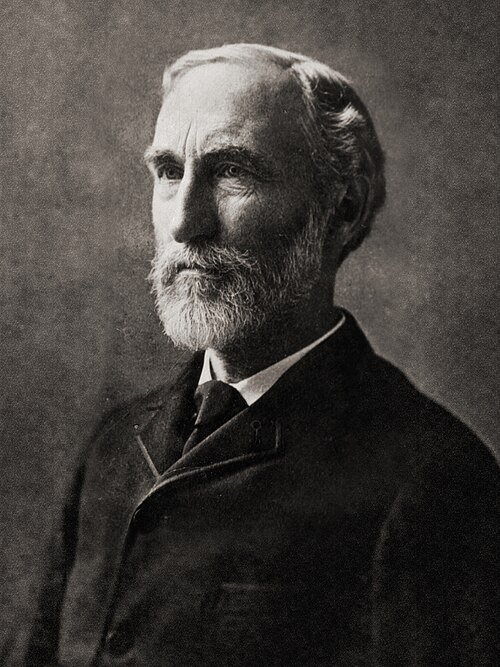
\includegraphics[width=\linewidth]{images/book3/gibbs.jpg}
\end{minipage}\hfill
\begin{minipage}[t]{0.76\linewidth}\vspace{0pt}
जोसायाह विलर्ड गिब्स (1839--1903), येल में गणितीय भौतिकी के प्राध्यापक, ने
1876 और 1878 के बीच \emph{विषमांगी पदार्थों के साम्य पर} (अंग्रेज़ी में) प्रकाशित
किया, जो एक छोटी अकादमी
के कार्यवृत्त में लगभग तीन सौ पृष्ठ हैं, जहाँ मुक्त ऊर्जा, रासायनिक विभव और
अगले अध्यायों का प्रावस्था नियम, सभी प्रकट होते हैं। 1890 के दशक में इसके अनुवाद
तक कम ही रसायनज्ञों ने इसे पढ़ा। (छायाचित्र: सार्वजनिक अधिकार-क्षेत्र, विकिमीडिया
कॉमन्स।)
\end{minipage}
\end{history}

\section{मानक अभिक्रिया गिब्स ऊर्जाएँ और ताप}

\begin{definition}[एलिंगम सन्निकटन]\label{def:b2:reaction-free-energy:ellingham-approximation}
\emph{एलिंगम सन्निकटन}\index{एलिंगम सन्निकटन}
$\Delta_r H^\circ$ और $\Delta_r S^\circ$ को ऐसे अंतराल में ताप से स्वतंत्र
मानता है जिसमें कोई अवस्था-परिवर्तन न हो। तब $\Delta_r G^\circ(T)
= \Delta_r H^\circ - T\Delta_r S^\circ$, $T$ में एक सरल रेखा है, जिसकी प्रवणता
$-\Delta_r S^\circ$ है।
\end{definition}

\begin{proposition}[ताप के सापेक्ष अवकलज]\label{prop:b2:reaction-free-energy:gibbs-helmholtz}
\[
  \frac{\dd\Delta_r G^\circ}{\dd T} = -\Delta_r S^\circ, \qquad
  \frac{\dd}{\dd T}\!\left(\frac{\Delta_r G^\circ}{T}\right) =
  -\frac{\Delta_r H^\circ}{T^2}\ \ \text{(गिब्स--हेल्महोल्ट्ज़)}, \qquad
  \frac{\dd\Delta_r S^\circ}{\dd T} = \frac{\Delta_r C^\circ_p}{T}.
\]
विशेष रूप से, \omterm{def:b2:reaction-free-energy:ellingham-approximation}{एलिंगम सन्निकटन} तब लागू होता है जब $\Delta_r C^\circ_p$
छोटा हो।
\end{proposition}

\begin{proof}
हर स्पीशीज़ के अपनी मानक अवस्था में होने पर, $G^\circ(T, \xi)$ के लिए $(\partial
G^\circ/\partial T)_\xi = -S^\circ$ (\cref{prop:b2:reaction-free-energy:dG})।
श्वार्ज़ प्रमेय से,
\[
  \frac{\dd\Delta_r G^\circ}{\dd T} = \partial_\xi\partial_T G^\circ =
  -\partial_\xi S^\circ = -\Delta_r S^\circ .
\] फिर $\frac{\dd}{\dd
T}(\Delta_r G^\circ/T) = \frac{-T\Delta_r S^\circ - \Delta_r G^\circ}{T^2} =
-\frac{\Delta_r H^\circ}{T^2}$। अंत में, हर स्पीशीज़ के लिए $\dd S^\circ_m = C^\circ_{p,m}\,\dd
T/T$ (\cref{prop:b2:reaction-free-energy:absolute-entropy}),
और वही संयोजन अंतिम संबंध देता है। यदि $\Delta_r C^\circ_p$
छोटा है, तो $\Delta_r H^\circ$ (किरखॉफ़) और $\Delta_r S^\circ$ मुश्किल से बदलते हैं।
\end{proof}

\begin{definition}[व्युत्क्रमण ताप]\label{def:b2:reaction-free-energy:inversion-temperature}
जब $\Delta_r H^\circ$ और $\Delta_r S^\circ$ का चिह्न एक ही हो, तो अभिक्रिया का
\emph{व्युत्क्रमण ताप}\index{व्युत्क्रमण ताप} वह
ताप है जिस पर $\Delta_r G^\circ$ का चिह्न बदलता है; \omterm{def:b2:reaction-free-energy:ellingham-approximation}{एलिंगम
सन्निकटन} में $T_i = \Delta_r H^\circ/\Delta_r S^\circ$।
\end{definition}

\begin{omfigure}
\begin{tikzpicture}
\begin{axis}[
  width=0.72\linewidth, height=5.6cm, xmin=0, xmax=1600, ymin=0, ymax=260,
  axis x line=bottom, axis y line=left, xlabel={$T$ (K)}, ylabel={\unit{kJ/mol}},
  tick label style={font=\small}, label style={font=\small}, clip=false]
\addplot[omThm, very thick] table[x=T, y=DrH] {figdata/out/bachelor-2-thermo-data-calcite.dat};
\addplot[omDef, very thick] table[x=T, y=TDrS] {figdata/out/bachelor-2-thermo-data-calcite.dat};
\node[omThm, anchor=south west, font=\small] at (axis cs:60,180) {$\Delta_r H^\circ = 178.3$};
\node[omDef, anchor=west, font=\small] at (axis cs:1600,257) {$T\Delta_r S^\circ$};
\draw[dotted] (axis cs:1110,0) -- (axis cs:1110,178.3);
\node[anchor=south west, font=\small] at (axis cs:1120,8) {$T_i = \qty{1110}{K}$};
\node[font=\scriptsize, align=center] at (axis cs:600,140) {$\Delta_r G^\circ > 0$:\\ कैल्साइट स्थायी};
\node[font=\scriptsize, align=center] at (axis cs:1470,206) {$\Delta_r G^\circ < 0$};
\end{axis}
\end{tikzpicture}

{\small \omterm{def:b2:reaction-free-energy:ellingham-approximation}{एलिंगम सन्निकटन} में \ce{CaCO3(s) -> CaO(s) + CO2(g)} के
एन्थैल्पी और एन्ट्रॉपी पद। \omterm{def:b2:reaction-free-energy:inversion-temperature}{व्युत्क्रमण ताप} से नीचे एन्थैल्पी
की लागत जीतती है और चूना पत्थर \qty{1}{bar} कार्बन डाइऑक्साइड के अंतर्गत
स्थायी रहता है; उससे ऊपर एन्ट्रॉपी पद जीतता है और चूना पत्थर विघटित होता है।}
% ledger: dfh:CaCO3_cr, dfh:CaO_cr, dfh:CO2, s0:CaCO3_cr, s0:CaO_cr, s0:CO2_g (computed in figdata/bachelor-2/thermo-data.py)
\end{omfigure}

\begin{omfigure}
\begin{tikzpicture}[font=\small]
  \draw[thick] (0,0) rectangle (8,4);
  \draw[thick] (4,0) -- (4,4) (0,2) -- (8,2);
  \node[above] at (2,4) {$\Delta_r H^\circ < 0$};
  \node[above] at (6,4) {$\Delta_r H^\circ > 0$};
  \node[left] at (0,3) {$\Delta_r S^\circ > 0$};
  \node[left] at (0,1) {$\Delta_r S^\circ < 0$};
  \node[align=center, omDef] at (2,3) {हर $T$ पर\\ ऊर्जामोची};
  \node[align=center, omProp] at (6,3) {$T_i$ से ऊपर\\ ऊर्जामोची};
  \node[align=center, omProp] at (2,1) {$T_i$ से नीचे\\ ऊर्जामोची};
  \node[align=center, omThm] at (6,1) {हर $T$ पर\\ ऊर्जाग्राही};
\end{tikzpicture}

{\small $\Delta_r G^\circ = \Delta_r H^\circ - T\Delta_r
S^\circ$ की चार स्थितियाँ (\omterm{def:b2:reaction-free-energy:ellingham-approximation}{एलिंगम सन्निकटन})। दहन ऊपर बाएँ खाने में हैं;
चूना पत्थर का विघटन और ठंडा पैक ऊपर दाएँ; अमोनिया का
संश्लेषण नीचे बाएँ।}
\end{omfigure}

\begin{method}[ताप $T$ पर मानक अभिक्रिया गिब्स ऊर्जा]\label{met:b2:reaction-free-energy:delta-g-standard}
\begin{enumerate}
  \item \qty{298.15}{K} की सारणियों से $\Delta_r H^\circ$ और
        $\Delta_r S^\circ$ परिकलित कीजिए।
  \item जाँचिए कि \qty{298}{K} और $T$ के बीच कोई स्पीशीज़ अवस्था नहीं बदलती;
        अन्यथा संक्रमण (एन्थैल्पी और एन्ट्रॉपी) जोड़िए या नई अवस्था से
        आरंभ कीजिए।
  \item \omterm{def:b2:reaction-free-energy:ellingham-approximation}{एलिंगम सन्निकटन} में $\Delta_r G^\circ(T) = \Delta_r H^\circ
        - T\Delta_r S^\circ$।
  \item जहाँ $\Delta_r C^\circ_p$ छोटा न हो या अंतराल लंबा हो, वहाँ
        सारणीबद्ध $\Delta_f G^\circ(T)$ का सीधे उपयोग कीजिए।
\end{enumerate}
\end{method}

\begin{example}[सन्निकटन की दो परीक्षाएँ]\label{ex:b2:reaction-free-energy:tests}
चूना पत्थर के लिए $\Delta_r C^\circ_p = 42.80 + 37.13 - 81.88 =
\qty{-2.0}{J/(K.mol)}$: सन्निकटन उत्कृष्ट है, और $\Delta_r
G^\circ = 178.3 - T \times 0.1606$ से $T_i = \qty{1110}{K}$ मिलता है। अमोनिया के लिए
$\Delta_r G^\circ(700) \approx -91.9 + 700 \times 0.1981 =
\qty{+46.8}{kJ/mol}$, जबकि सारणियाँ $2\Delta_f G^\circ(\ce{NH3}, 700) =
\qty{+54.4}{kJ/mol}$ देती हैं: यहाँ $\Delta_r C^\circ_p = \qty{-44}{J/(K.mol)}$ है और
त्रुटि \qty{8}{kJ/mol} है, जो उस ताप पर साम्य स्थिरांक में 4 का
गुणक है।
% ledger: cp:CaO_cr.298, cp:CO2_g.298, cp:CaCO3_cr.298, janafG:NH3.700 (computed in figdata/bachelor-2/thermo-data.py)
\end{example}

\section{अभ्यास}

\begin{exercise}[$\star$]\label{exo:b2:reaction-free-energy:1}
इनके लिए $\Delta_r S^\circ$ के चिह्न का पूर्वानुमान कीजिए: (a) \ce{2H2(g) + O2(g) -> 2H2O(l)};
(b) \ce{CaCO3(s) -> CaO(s) + CO2(g)}; (c) \ce{N2O4(g) -> 2NO2(g)};
(d) \ce{Ag+(aq) + Cl-(aq) -> AgCl(s)}; (e) \ce{H2O(s) -> H2O(l)};
(f) \ce{H2(g) + Cl2(g) -> 2HCl(g)}.
\end{exercise}

\begin{exercise}[$\star$]\label{exo:b2:reaction-free-energy:2}
अमोनिया के संश्लेषण, \ce{N2(g) + 3H2(g) -> 2NH3(g)}, के लिए \qty{298.15}{K} पर
$\Delta_r S^\circ$ और $\Delta_r G^\circ$ परिकलित कीजिए, $\Delta_r
H^\circ = \qty{-91.9}{kJ/mol}$ और अध्याय की एन्ट्रॉपियों के साथ। क्या यह
\omterm{def:b2:reaction-free-energy:exergonic}{ऊर्जामोची} है?
\end{exercise}

\begin{exercise}[$\star$]\label{exo:b2:reaction-free-energy:3}
\ce{H2(g) + 1/2O2(g) ->
H2O(l)} का $\Delta_r G^\circ(\qty{298.15}{K})$ परिकलित कीजिए, $\Delta_f H^\circ(\ce{H2O}, \text{l}) = \qty{-285.83}{kJ/mol}$
और मानक एन्ट्रॉपियों \ce{H2(g)} 130.68, \ce{O2(g)} 205.15,
\ce{H2O(l)} \qty{69.95}{J/(K.mol)} से। यह मान द्रव जल की मानक संभवन
\omterm{def:b2:reaction-free-energy:gibbs-energy}{गिब्स ऊर्जा} क्यों है?
% ledger: dfh:H2O-l, s0:H2_g, s0:O2_g, s0:H2O_l
\end{exercise}

\begin{exercise}[$\star$]\label{exo:b2:reaction-free-energy:4}
ज़िंक की एन्ट्रॉपी वाले चित्र से \qty{298}{K} और \qty{1000}{K} पर उसकी \omterm{def:b2:reaction-free-energy:standard-entropy}{मानक मोलर
एन्ट्रॉपी}, और गलनांक तथा क्वथनांक पर उसके उछाल पढ़िए।
उसकी गलन और वाष्पन एन्थैल्पियाँ निकालिए।
\end{exercise}

\begin{exercise}[$\star\star$]\label{exo:b2:reaction-free-energy:5}
\qty{298.15}{K} पर \ce{H2O(l) -> H2O(g)} के लिए अध्याय की सारणियों से $\Delta_r H^\circ$,
$\Delta_r S^\circ$ और $\Delta_r G^\circ$ परिकलित कीजिए।
समझाइए कि \qty{298}{K} पर $\Delta_r S^\circ \neq \Delta_r H^\circ/T$ क्यों है,
धनात्मक $\Delta_r G^\circ$ का क्या अर्थ है, और \omterm{def:b2:reaction-free-energy:ellingham-approximation}{एलिंगम सन्निकटन} में
उस ताप का आकलन कीजिए जिस पर द्रव जल और \qty{1}{bar} पर उसकी वाष्प
साम्य में होते हैं। क्वथनांक से तुलना कीजिए।
\end{exercise}

\begin{exercise}[$\star\star$]\label{exo:b2:reaction-free-energy:6}
\ce{N2O4(g) -> 2NO2(g)} के लिए $\Delta_r H^\circ = \qty{57.1}{kJ/mol}$ और
$\Delta_r S^\circ = \qty{175.7}{J/(K.mol)}$। \omterm{def:b2:reaction-free-energy:inversion-temperature}{व्युत्क्रमण
ताप} परिकलित कीजिए, और समझाइए कि भूरी गैस \ce{NO2} की सीलबंद नली
बर्फ़ में ठंडी करने पर फीकी क्यों पड़ जाती है।
\end{exercise}

\begin{exercise}[$\star\star$]\label{exo:b2:reaction-free-energy:7}
किसी अभिक्रिया के लिए \qty{300}{K} पर $\Delta_r G^\circ = \qty{-12.0}{kJ/mol}$
और \qty{400}{K} पर $\qty{-4.0}{kJ/mol}$ है। \omterm{def:b2:reaction-free-energy:ellingham-approximation}{एलिंगम सन्निकटन} में
$\Delta_r H^\circ$ और $\Delta_r S^\circ$ ज्ञात कीजिए, और
गिब्स--हेल्महोल्ट्ज़ संबंध की जाँच कीजिए।
\end{exercise}

\begin{exercise}[$\star\star$]\label{exo:b2:reaction-free-energy:8}
मेथेन के संभवन, \ce{C(s) + 2H2(g) ->
CH4(g)}, का \qty{298.15}{K} पर $\Delta_r G^\circ$ परिकलित कीजिए, $\Delta_f H^\circ = \qty{-74.87}{kJ/mol}$
और एन्ट्रॉपियों \ce{C} (ग्रेफ़ाइट) 5.74, \ce{H2} 130.68, \ce{CH4}
\qty{186.25}{J/(K.mol)} से। किस ताप से ऊपर मेथेन मानक दाब पर अपने
तत्वों के सापेक्ष अस्थायी हो जाती है?
% ledger: dfh:CH4_g, s0:C_gr, s0:H2_g, s0:CH4_g
\end{exercise}

\begin{exercise}[$\star\star$]\label{exo:b2:reaction-free-energy:9}
कोई हैलोऐल्केन किसी क्षारक से प्रतिस्थापन या विलोपन द्वारा अभिक्रिया करता है।
2-ब्रोमोप्रोपेन और हाइड्रॉक्साइड के लिए दोनों अभिक्रियाएँ लिखिए। $\Delta_r
H^\circ(\text{विलोपन}) - \Delta_r H^\circ(\text{प्रतिस्थापन}) =
\qty{+40}{kJ/mol}$ और $\Delta_r S^\circ(\text{विलोपन}) - \Delta_r
S^\circ(\text{प्रतिस्थापन}) = \qty{+90}{J/(K.mol)}$ (परिमाण की कोटियाँ) के साथ,
ज्ञात कीजिए कि किस ताप से ऊपर दोनों में विलोपन अधिक \omterm{def:b2:reaction-free-energy:exergonic}{ऊर्जामोची} बन जाता है,
और अणुओं की संख्या की भूमिका समझाइए।
\end{exercise}

\begin{exercise}[$\star\star\star$]\label{exo:b2:reaction-free-energy:10}
क्रिस्टलीय कार्बन मोनॉक्साइड \qty{0}{K} पर शून्य एन्ट्रॉपी तक नहीं पहुँचता: हर
अणु लगभग यादृच्छिक रूप से CO या OC के रूप में बैठ सकता है, क्योंकि दोनों अभिविन्यासों की
ऊर्जा लगभग समान है। बोल्ट्ज़मान का सूत्र $S = k_B\ln W$ स्वीकार करते हुए, जहाँ
$W$ विन्यासों की संख्या है (तृतीय वर्ष के खंड में गिनी गई), अवशिष्ट
मोलर एन्ट्रॉपी परिकलित कीजिए। तृतीय नियम इस क्रिस्टल पर
लागू क्यों नहीं होता?
\end{exercise}

\begin{exercise}[$\star\star\star$]\label{exo:b2:reaction-free-energy:11}
दिखाइए कि यदि $\Delta_r C^\circ_p$ एक अचर $c$ है, तो
$\Delta_r S^\circ(T) = \Delta_r S^\circ(T_0) + c\ln(T/T_0)$ और
$\Delta_r G^\circ(T) = \Delta_r H^\circ(T_0) - T\Delta_r S^\circ(T_0) +
c\,[T - T_0 - T\ln(T/T_0)]$। इसे चूना पत्थर ($c =
\qty{-2.0}{J/(K.mol)}$) पर \qty{1100}{K} पर लागू कीजिए, और
\omterm{def:b2:reaction-free-energy:ellingham-approximation}{एलिंगम सन्निकटन} की त्रुटि मापिए।
\end{exercise}

\begin{exercise}[$\star\star\star$]\label{exo:b2:reaction-free-energy:12}
टाइटेनियम उसके ऑक्साइड, रूटाइल, से उसके क्लोराइड के माध्यम से बनाया जाता है। (a)
\ce{TiO2(s) +
2Cl2(g) -> TiCl4(g) + O2(g)} के \qty{298}{K} पर $\Delta_r H^\circ$ और $\Delta_r S^\circ$ परिकलित कीजिए,
\ce{TiO2} ($-944.0$ \unit{kJ/mol},
\qty{50.62}{J/(K.mol)}) और \ce{TiCl4(g)} ($-763.2$, 353.2) के साथ, और \omterm{def:b2:reaction-free-energy:ellingham-approximation}{एलिंगम सन्निकटन} में
\qty{1000}{K} पर इसका $\Delta_r G^\circ$।
(b) कार्बन मिलाया जाता है: \ce{C(s) + O2(g) -> CO2(g)}, $\Delta_r H^\circ =
\qty{-393.5}{kJ/mol}$, $\Delta_r S^\circ = \qty{+2.9}{J/(K.mol)}$। दोनों अभिक्रियाओं के
योग का $\Delta_r G^\circ(\qty{1000}{K})$ परिकलित कीजिए और
समझाइए कि दूसरी अभिक्रिया पहली को कैसे चलाती है।
% ledger: dfh:TiO2_cr, s0:TiO2_cr, dfh:TiCl4_g, s0:TiCl4_g, s0:Cl2_g, s0:O2_g, s0:C_gr, s0:CO2_g
\end{exercise}

\section{समस्या: चूने की भट्ठी}

\begin{problem}[{सप्ताहांत समस्या --- किसी विघटन की एन्ट्रॉपी और
एन्थैल्पी, ताप के सापेक्ष उसकी गिब्स ऊर्जा, भट्ठी में विकास
निकष, और एक टन चूने की ऊर्जा और कार्बन
डाइऑक्साइड}]
\label{pb:b2:reaction-free-energy:1}
चूना, \ce{CaO}, चूना पत्थर, \ce{CaCO3}, को भट्ठी में गर्म करके बनाया जाता है।
\qty{298.15}{K} पर आँकड़े: $\Delta_f H^\circ$ (\unit{kJ/mol}) \ce{CaCO3(s)}
$-1206.92$, \ce{CaO(s)} $-635.09$, \ce{CO2(g)} $-393.51$; $S^\circ_m$
(\unit{J/(K.mol)}) 92.9, 39.75, 213.79; $C^\circ_{p,m}$ (\unit{J/(K.mol)})
81.88, 42.80, 37.13। मोलर द्रव्यमान: \ce{CaO} \qty{56.08}{g/mol}, \ce{CO2}
\qty{44.01}{g/mol}, \ce{CH4} \qty{16.04}{g/mol}; मेथेन का दहन,
जल वाष्प के रूप में, $\Delta_r H^\circ = \qty{-802.3}{kJ/mol}$।
% ledger: dfh:CaCO3_cr, dfh:CaO_cr, dfh:CO2, s0:CaCO3_cr, s0:CaO_cr, s0:CO2_g, cp:CaCO3_cr.298, cp:CaO_cr.298, cp:CO2_g.298

\medskip
\noindent\textbf{भाग I --- कमरे के ताप पर।}
\begin{enumerate}
  \item चूना पत्थर का विघटन लिखिए।
  \item $\Delta_r H^\circ(\qty{298}{K})$ परिकलित कीजिए। क्या अभिक्रिया \omterm{def:b2:reaction-enthalpy:exothermic}{ऊष्माक्षेपी} है?
  \item $\Delta_r S^\circ(\qty{298}{K})$ परिकलित कीजिए और उसका चिह्न समझाइए।
  \item $\Delta_r G^\circ(\qty{298}{K})$ परिकलित कीजिए।
  \item क्या कमरे के ताप पर \qty{1}{bar} कार्बन डाइऑक्साइड के अंतर्गत चूना पत्थर
        स्थायी है? चूना पत्थर की चट्टानें क्यों टिकी रहती हैं?
  \item $\Delta_r C^\circ_p$ परिकलित कीजिए, और बताइए कि $\Delta_r H^\circ$ और $\Delta_r S^\circ$ की
        ताप-निर्भरता के लिए इसका क्या अर्थ है।
\end{enumerate}

\medskip
\noindent\textbf{भाग II --- तापन।}
\begin{enumerate}[resume]
  \item \omterm{def:b2:reaction-free-energy:ellingham-approximation}{एलिंगम सन्निकटन} में $\Delta_r G^\circ(T)$ लिखिए।
  \item इसे \qty{1000}{K} और \qty{1300}{K} पर परिकलित कीजिए।
  \item \omterm{def:b2:reaction-free-energy:inversion-temperature}{व्युत्क्रमण ताप} $T_i$ परिकलित कीजिए।
  \item इस व्यंजक पर गिब्स--हेल्महोल्ट्ज़ संबंध की जाँच कीजिए।
  \item \cref{exo:b2:reaction-free-energy:11} के सूत्र से,
        $\Delta_r G^\circ$ में $T_i$ पर होने वाले उस परिवर्तन का आकलन कीजिए जो
        $\Delta_r C^\circ_p$ के कारण है, और $T_i$ के परिणामी विस्थापन का भी।
\end{enumerate}

\medskip
\noindent\textbf{भाग III --- भट्ठी।}
इस भाग में ठोसों के ऊपर कार्बन डाइऑक्साइड \qty{1}{bar} पर है, जिससे
$\Delta_r G = \Delta_r G^\circ$।
\begin{enumerate}[resume]
  \item \qty{1000}{K} पर विकास निकष क्या कहता है? और
        \qty{1300}{K} पर?
  \item चूने और \qty{1}{bar} कार्बन डाइऑक्साइड के मिश्रण को
        $T_i$ से नीचे ठंडा करने पर क्या होता है?
  \item \qty{1300}{K} पर विघटित चूना पत्थर के प्रति मोल कितनी एन्ट्रॉपी उत्पन्न
        होती है?
  \item भट्ठियों में दहन गैसें बहती हैं, जिनमें कार्बन डाइऑक्साइड कम होती है।
        अगले अध्याय से पहले अनुमान लगाइए कि क्या इससे
        विघटन में सहायता मिलती है।
\end{enumerate}

\medskip
\noindent\textbf{भाग IV --- एक टन चूना।}
\begin{enumerate}[resume]
  \item एक टन में चूने की मात्रा परिकलित कीजिए।
  \item प्रति टन चूना अभिक्रिया द्वारा अवशोषित ऊष्मा परिकलित कीजिए
        ($\Delta_r H^\circ$ को स्थिर लीजिए)।
  \item प्रति टन चूना, चूना पत्थर द्वारा मुक्त कार्बन डाइऑक्साइड का द्रव्यमान
        परिकलित कीजिए।
  \item ऊष्मा मेथेन के दहन से आती है, जिसकी उपयोगी दक्षता
        50\,\% है। प्रति टन चूना जलाई गई मेथेन का द्रव्यमान परिकलित कीजिए।
  \item इस मेथेन से आने वाली कार्बन डाइऑक्साइड परिकलित कीजिए।
  \item प्रति टन चूना कुल कार्बन डाइऑक्साइड परिकलित कीजिए, और उसमें
        स्वयं चूना पत्थर का अंश।
  \item स्वच्छतर ईंधन इन उत्सर्जनों का केवल एक भाग ही क्यों घटा सकता है?
  \item वह ताप बताइए जिससे ऊपर चूना पत्थर \qty{1}{bar} कार्बन
        डाइऑक्साइड के अंतर्गत विघटित होता है।
\end{enumerate}
\end{problem}
